\clearpage\newpage

\subsection{CC theta Matching}

This, and the following CC $\phi$ and Time Matching procedures, are based on a study
\cite{bib:ccmatch},\cite{bib:pc_fxpun}, \cite{bib:pc_osi} of the \v Cerenkov response function.

The CC $\theta$ matching requires the candidate electrons tracks to match
a signal in the CC. The CC segments (one pmt from the right and the corresponding from the left,
constitute a segment) and mirrors are placed along the CLAS polar angle.
Since the torus magnetic field bend the electrons toward the beamline, it's convenient
not to use the track $\theta$ angle at the vertex but the angle $\theta_{CC}$ of the point of
intersection of the track with the CC plane. These are the details of the  $\theta_{CC}$
calculation:
\begin{itemize}
    \item [1.] The intersection of the track with the TOF plane  $\vec{P}_0$ is considered (DCPB bank).
    \item [2.] The normalized direction of the track $\vec{n}$ of the track to the TOF plane is considered (DCPB bank).
    \item [3.] The line representing the un-bending track is then $\vec{P} = \vec{P}_0 - t\vec{n}$
    (the minus sign accounts for the fact that the CC is before the TOF).
    \item [4.] The CC plane equation is considered: $Ax+By+Cz+D=0$, with
    $A=-0.000784$, $B=0$, $C=-0.00168$, and $D=1$ \cite{bib:ccmatch}. This is also represented
    by the vector $\vec{S} = (A, B, C)$
    \item [5.] Substituting the line equation in the plane equation one finds the distance of the path length from the
    intersection of the track with the TOF plane and the intersection of the track with the CC plane:
    $$t=\frac{\vec{S} \cdot \vec{P}_0}{\vec{S} \cdot \vec{n}}$$
\end{itemize}
There should be one to one correspondence between $\theta_{CC}$ and segment number for real tracks, while
background noise and accidentals should show no such correlation.
For each segment, the $\theta_{CC}$ distribution is fitted with a gaussian + second order
polynomial distribution to determine its mean and width. Examples of these fits can be found
in Fig.~\ref{fig:ccm_slices}. Events that have $\mu - 4\sigma < \theta_{CC} < \mu - 3\sigma$
pass the cut (this accounts for the distribution not being completely symmetric around the mean).
The overall $\theta_{CC}$ versus segment distribution and the lower/upper limits
are shown in Fig.~\ref{fig:ccm_theta}.

There are two exception to this cut:
\begin{itemize}
    \item [1.] The first and last segments distributions is hard to fit. The cut in this case is ignored.
    \item [2.] If both (left and right) photomultipliers have a signal the track is kept.
\end{itemize}
The events that fall in this category can be seen in the bottom right panel in Fig.~\ref{fig:ccm_theta}.

\begin{figure}[ht]
    \vspace{-1cm}
    \centering
    \includegraphics[width=0.44\textwidth]{img/slice-06_cut-01-ts_sector-1}
    \includegraphics[width=0.44\textwidth]{img/slice-06_cut-01-ts_sector-1}
    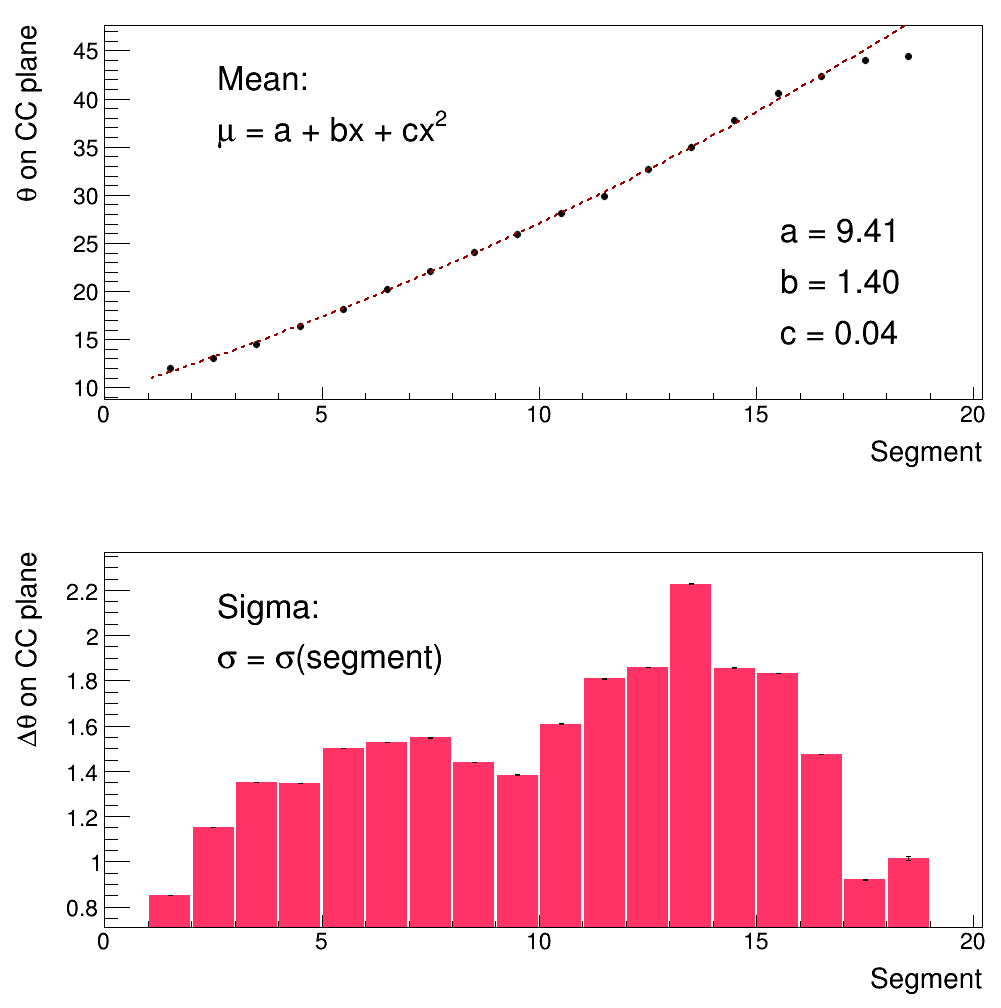
\includegraphics[width=0.88\textwidth]{img/cut-01-tmp_sector-1}
    \caption{Top panels: $\theta_{CC}$ for two segments in sector 1, and gaussian + second order
    polynomial fit. The distribution is slightly asymmetric to the
    left, so the lower limit was $4\sigma$ while the upper limit
    was $3\sigma$.
    Bottom Panels: the mean distribution is fitted with a third order
    polynomial.  }
    \label{fig:ccm_slices}
\end{figure}


\begin{figure}[ht]
    \centering
    \includegraphics[width=0.98\textwidth]{img/cut-01-tmc_sector-1}
    \caption{$\theta_{CC}$ versus Segment for Sector 1. The $\theta_{CC}$
        distribution for each segment is fitted with a gaussian +
        second order polynomial distribution to determine its mean
        and width. Events that have $\mu - 4\sigma < \theta_{CC} < \mu - 3\sigma$
        pass the cut.
        Top left: all events. Top right: events with calorimeter cuts applied
        (notice that these cuts remove $74 \,^{\circ\!\!}/\!_\circ$ of the data).
        Bottom left: events with the negative calorimeter cuts applied.
        Bottom right: all cuts applied. Notice that the CC matching cut
        only removes $7  \,^{\circ\!\!}/\!_\circ$ of the events with
        the calorimeter cuts already applied.}
    \label{fig:ccm_theta}
\end{figure}
